\documentclass{article}
\usepackage{ctex}
\usepackage{amsmath}
\usepackage{graphicx}
\usepackage{wrapfig}
\usepackage{caption}
\usepackage[top=0.8in, bottom=0.8in,left=0.8in, right=0.8in]{geometry}
\usepackage{float} 
\usepackage{subfigure}
\usepackage{subcaption}
\usepackage{bm}
\xeCJKsetup{CJKmath=true} 

\begin{document}
\section*{重力弹球(80分)}

\subsection*{PART.A\ \ 一些准备工作}
\begin{itemize}
    \item[(A.1)]
    \begin{equation}\vec{n}|_p=\dfrac{\vec{\nabla}\cdot M|_p}{\left|\vec{\nabla}\cdot M|_p\right|}=\dfrac{(-\dfrac{x}{2f},-\dfrac{y}{2f},1)}{\sqrt{1+\dfrac{x^2+y^2}{4f^2}}}\end{equation}
    \item[(A.2)]
    \begin{equation}v_{\parallel}=\sqrt{v_{x}^{2}+v_{y}^{2}},z=v_z t-\frac{1}{2}gt^{2},x'=v_{\parallel}t\end{equation}
    \begin{equation}z=\frac{v_z}{v_{\parallel}}x'-\dfrac{1}{2}g\dfrac{x'^{2}}{v_{\parallel^2}}\end{equation}
    \begin{equation}p=\frac{v_{\parallel}^{2}}{g}\end{equation}
    \begin{equation}F=\frac{v_x^2+v_y^2}{2g}\end{equation}
    \item[(A.3)]
    \begin{equation}\vec{v'}=\vec{v}-2(\vec{n}|_P\cdot\vec{v})\cdot\vec{n}|_P\end{equation}
    \item[(A.4)]
    \begin{equation}\dfrac{L_z}{m}=(\vec{r}\times\vec{v})z=(\vec{r}\times\vec{v'})_z-2(\vec{n}|_P\cdot\vec{v})(\vec{r}\times\vec{n})_z=(\vec{r}\times\vec{z})_z\end{equation}
    利用了$(\vec{r}\times\vec{n}|_P)_z=0$
\end{itemize}
\subsection*{PART.B\ \ 一种特殊情况}
\begin{itemize}
    \item[(B.1)]\begin{equation}\tan\dfrac{\theta}{2}=\frac{v_{r}}{v_{\phi}}\end{equation}
    \item[(B.2)]由于碰撞点在同一水平圆上,有
    \begin{equation}\begin{cases}2r_{0}\sin\dfrac{\theta}{2}=\sqrt{v_{r}^{2}+v_{\phi}^{2}}t\\v_{z}t-\dfrac{1}{2}gt^{2}=0\end{cases}\end{equation}
    \begin{equation}z_{z}=\dfrac{1}{2}g\frac{2r_{0}\sin\dfrac{\theta}{2}}{\sqrt{v_{r}^{2}+v_{\phi}^{2}}}=\dfrac{gr_{0}\sin\dfrac{\theta}{2}}{\sqrt{v_{r}^{2}+v_{\phi}^{2}}}\end{equation}
    由于碰撞撞点要一直在这个圆上,所以入射速度与出射速度与水平方向夹角不变
    \begin{equation}\dfrac{v_r}{v_z}=\dfrac{r_0}{2f}\end{equation}
    由$(7),(8)$式
    \begin{equation}v_z=\dfrac{zf}{r_{0}}v_r=\frac{gr_{0}\sin\dfrac\theta2}{v_r\sqrt{1+\cot^{2}\dfrac\theta2}}=\dfrac{gr_{0}\sin^{2}\dfrac\theta2}{v_r}\end{equation}
    \begin{equation}\Rightarrow\quad v_r^{2}=\dfrac{gr_{0}^{2}}{2f}\sin^{2}\frac{\theta}{2}=\dfrac{gr_{0}^{2}}{2f}\dfrac{1-\cos\theta}{2}\end{equation}
    解得
    \begin{equation}\begin{cases}v_{r}=\dfrac{r_{0}}{2}\sqrt{\dfrac{g}{f}(1-\cos\theta)}\\v_{z}=\sqrt{gf(1-\cos\theta)}\\v_{\phi}=\dfrac{r_{0}}{2}\sqrt{\dfrac{g}{f}(1+\cos\theta)}\end{cases}\end{equation}
    \item[(B.3)]离开圆心$r$处有
    \begin{equation}\begin{cases}x^{\prime}=r_0\sin\dfrac{\theta}{2}-\sqrt{r^2-r_0^2\cot^2\dfrac{\theta}{2}}=\sqrt{v_{r}^2+v_{\phi}^2}t\\
        z^{\prime}=v_zt-\dfrac{1}{2}gt^2=\dfrac{v_zx}{\sqrt{v_{r}^2+v_{\psi}^2}}-\dfrac12g\dfrac{x^2}{v_{r}^2+v_{\psi}^2}\end{cases}\end{equation}
        化简后可得与$\theta$无关
        \begin{equation}z=z^{\prime}+\frac{r_{0}^{2}}{4y}-f=\frac{r_{0}^{2}}{4y}-\frac{fr^{2}}{r_{0}^{2}}\qquad r\in[v_{0}\cos\dfrac\theta2,v_{0}]\end{equation} 
\end{itemize}
\subsection*{PART.C\ \ 二维抛物线内的弹球}
\begin{itemize}
    \item[(C.1)]
    \begin{equation}x=v\cos\alpha t\end{equation}
    \begin{equation}z=v\sin\alpha t-\dfrac 12gt^2=x\tan\alpha-\dfrac 12gt^2=x\tan\alpha-\dfrac 12g\dfrac{x^2}{v^2\cos^2\alpha}\end{equation}
    \begin{equation}f=\frac{v^2\cos^2\alpha}{2g}\end{equation}
    \begin{equation}x=\dfrac{\tan\alpha}{-2(-\dfrac12g\dfrac1{v^2\sin\alpha})}=\dfrac{v^2\sin\alpha\cos\alpha}{g}=\frac{v^2\sin2\alpha}{2g}\end{equation}
    \item[(C.2)]由抛物线的光学性质得
    \begin{center}
        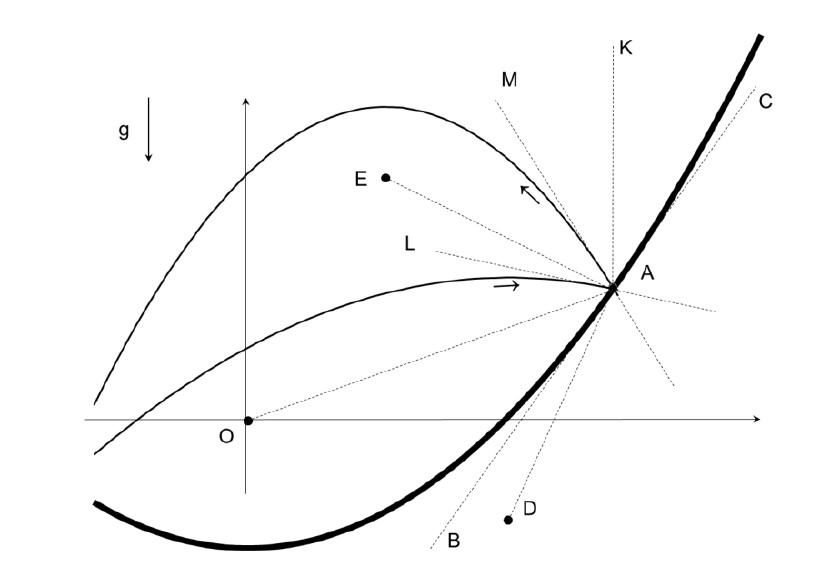
\includegraphics[scale=0.3]{img/0017.4.jpg}\par
    \end{center}
    \begin{equation}\angle EAM=\angle MAK\end{equation}
    \begin{equation}\angle DAL=\angle LAK\end{equation}
    \begin{equation}\angle EAO=-\angle EAM+\angle DAM=-\angle MAK+\angle OAM\end{equation}
    \begin{equation}\angle DAO=\angle DAL-\angle DAL=\angle LAK-\angle DAL\end{equation}
    \begin{equation}\angle EAO=-(\angle MAK+\angle MAK)+\angle DAM+\angle OAL=-\angle MAL+\angle MAL=0\end{equation}
    \item[(C.3)]
    \begin{equation}H=z_{0}+\dfrac{\dfrac{1}{2}mv_z^{2}}{mg}+\frac{v^{2}\cos^{2}\alpha}{2g}=z_{0}+\frac{v^{2}}{2g}\end{equation}
    \begin{equation}与碰撞前后无关\end{equation}
    \item[(C.4)]由于
    \begin{equation}\angle EAO=\angle OAD,AE=AO\end{equation}
    可得
    \begin{equation}\triangle OAE\cong\triangle OAD\end{equation}
    故
    \begin{equation}OE=OD\end{equation}
    \item[(C.5)] 以轨迹焦点为原点
    \begin{equation}\begin{cases}z^{\prime}=z-R\sin\alpha\\x^{\prime}=x-R\cos\alpha\end{cases}\end{equation}
    而
    \begin{equation}f=\dfrac12(H-R\sin\alpha)\end{equation}
    \begin{equation}2(H-R\sin\alpha)(z-R\sin\alpha)=-(x-R\cos\alpha)^2+(H-R\sin\alpha)^2\end{equation}
    设\begin{equation}S(x,z,\alpha)=2R(z\sin\alpha+x\cos\alpha)+H^2-x^2-R^2-2Hz=0\end{equation}
    \begin{equation}\frac{\partial S}{\partial\alpha}=2R\left(z\cos\alpha-x\sin\alpha\right)=0\end{equation}
    \begin{itemize}
        \item[1)]\begin{equation}\sin\alpha=\dfrac{z}{\sqrt{x^2+z^2}}\quad\cos\alpha=\dfrac{x}{\sqrt{x^2+z^2}}\end{equation}
        \begin{equation}-2Hz+2R\sqrt{x^2+z^2}\quad+H^2-x^2+R^2=0\end{equation}
        \item[2)]\begin{equation}\sin\alpha=-\dfrac{z}{\sqrt{x^2+z^2}}\quad\cos\alpha=-\dfrac{x}{\sqrt{x^2+z^2}}\end{equation}
        \begin{equation}-2Hz-2R\sqrt{x^2+z^2}+H^2-x^2-R^2=0\end{equation}
    \end{itemize}
    \item[(C.6)]过$B,C$作竖直线,由抛物线的第二定义
    \begin{equation}\overline{BA}+\overline{BO}=\overline{BM}+\overline{BD}=\overline{EG}\end{equation}
    \begin{equation}\overline{CA}+\overline{CO}=\overline{CE}+\overline{CG}=\overline{DM}\end{equation}
    \begin{equation}到O,A距离为定值\end{equation}
\end{itemize}
% \subsection*{参考文献}
% \bibliographystyle{plain}
% \bibliography{citation.bib}
\begin{thebibliography}{99}  

    % \bibitem{ref1}郭莉莉,白国君,尹泽成,魏惠芳. “互联网+”背景下沈阳智慧交通系统发展对策建议[A]. 中共沈阳市委、沈阳市人民政府.第十七届沈阳科学学术年会论文集[C].中共沈阳市委、沈阳市人民政府:沈阳市科学技术协会,2020:4.
    % \bibitem{ref2}陈香敏,魏伟,吴莹. “文化+人工智能”视阈下文化创意产业融合发展实践及路径研究[A]. 中共沈阳市委、沈阳市人民政府.第十七届沈阳科学学术年会论文集[C].中共沈阳市委、沈阳市人民政府:沈阳市科学技术协会,2020:4.
    % \bibitem{ref3}田晓曦,刘振鹏,彭宝权. 地方高校开展教育人工智能深度融合的路径探究[A]. 中共沈阳市委、沈阳市人民政府.第十七届沈阳科学学术年会论文集[C].中共沈阳市委、沈阳市人民政府:沈阳市科学技术协会,2020:5.
    % \bibitem{ref4}柏卓君,潘勇,李仲余.彩色多普勒超声在早期胚胎停育诊断中的应用[J].影像研究与医学应用,2020,4(18):129-131.
    % \bibitem{ref5}杨芸.我院2018年人血白蛋白临床应用调查与分析[J].上海医药,2020,41(17):34-35+74.

    \bibitem{Jaud2023GravitationalB}
    D.~Jaud.
    \newblock Gravitational billiards -- bouncing inside a paraboloid cavity.
    \newblock {\em arXiv: math.DS}, 2023.
    
    \bibitem{Masalovich2020BilliardsIA}
    S.~Masalovich.
    \newblock Billiards in a gravitational field: A particle bouncing on a
      parabolic and right angle mirror.
    \newblock {\em arXiv: Optics}, 2020.
    
    
    \end{thebibliography}
\end{document}

